%% La letra n con tilde es: 'n.
\chapter{Background}\label{background}

In this chapter the fundamental concepts related this work are presented:
Formal definitions referring to fuzzy systems, contextual factors and
recommender system techniques used by the proposed method.
%--------------------------------------------------------------
%Agregue la seccion de logica difusa del articulo que me mando.

\section{Production systems and fuzzy models}

A central aspect of the proposed method is the use of both fuzzy logic and
fuzzy inference systems, in this section formal definitions of
these models of knowledge representation are presented.  

\subsection{Traditional Production Systems}
Production Systems represent knowledge in form of rules, which specify
actions that will be executed when certain conditions are met. In these 
systems Experts in a certain domain identify a set of rules based 
on their experience to
resolve different kinds of problems. Also known as rule based systems,
many implementations consist of mainly these three
components \cite{brachman1992knowledge} \cite{konar2006computational}:
\begin{enumerate}   
\item \textbf{Production Rules (PR)}. A set of
production rules (also known as \textit{IF-THEN} rules) having a two part
structure; the antecedent, conformed by a set of conditions and a
consequent set of actions. 
\item \textbf{Working Memory (WM)}.
Represents the current knowledge or facts that are known to be true so
far. These facts are tested by the antecedent conditions of the rules
and the consequent part can change them. 
\item \textbf{Inference Engine (IE)}. 
This interpreter matches the conditions in the
production rules with the data/instantiations found in the WM,
deriving new consequences.
\end{enumerate}
The basic operation of these systems is described as a cycle of 
three steps \cite{brachman1992knowledge}:
\begin{enumerate}
\item \textbf{Recognize}: Find which rules are satisfied by 
the current WM. The antecedent part of the productions consists 
of a set of clauses connected by AND operators, when all these 
clauses have matching data on the WM the production has a chance 
of firing.
\item \textbf{Conflict Resolution}: Only one production can be 
fired at a time, so when two or more rules can be fired concurrently 
a conflict occurs. Among the production rules found in the first 
step, choose which rules should fire.
\item \textbf{Actions}: Change the working memory by performing 
the actions specified in the consequent part of all the rules 
selected in the second step. Changes occur by adding or 
deleting elements of the WM.
\end{enumerate}
This cycle continues until no further production rules can be fired.
This control strategy is data driven because whenever the antecedent
part is satisfied the rule is recognized, this strategy is also named
chain-forward. Other strategy is chain-backward in which case the work
is done from the conclusion to the facts, to chain-backward, goals in
the WM are matched against consequents of the production
rules.\\A drawback that has been recognized in these traditional
productions systems, is that some times rules are not fired in the
Recognize step because no appropriate match exists in the WM. Partial
matching of rules is not possible and this can be a limitation in some
systems because premature termination of the cycle is not desired. An
approach to handle partial matching is using fuzzy logic
\cite{konar2006computational}. In the next section a review of the
extension of production systems with fuzzy logic is presented.\\

\subsection{Fuzzy Production Rules}

Fuzzy production rules use fuzzy logic sets to characterize the
variables and terms used in the propositions of the rules. Fuzzy
production rules or fuzzy \textit{IF-THEN} rules are expressions of
the form \textit{IF} antecedent \textit{THEN} consequent, where the
antecedent is a proposition of the form \textit{"x is A"} where
\textit{x} is a linguistic variable and \textit{A} is a linguistic
term. The truth value of this proposition is based on the matching
degree between \textit{x} and \textit{A}. Propositions are connected
by \textit{AND}, \textit{OR} and \textit{NOT} operators. Some
implementations of fuzzy rule-based systems also include other kinds
of data types in their propositions, for example the FLOPS system
includes fuzzy numbers, hedges, and non fuzzy data types (integers,
strings and float) \cite{siler2005fuzzy}. Depending on the form of the
consequent, two main types of fuzzy production systems are
distinguished \cite{babuvska1996fuzzy}:
\begin{itemize}  
\item \textbf{Linguistic fuzzy model}: where both the antecedent 
and consequent are fuzzy propositions.
\item \textbf{Takagi-Sugeno fuzzy model}: the antecedent is a fuzzy 
proposition; the consequent is a crisp function.
\end{itemize}  
As before, other non-fuzzy consequents can also be implemented, like
the execution of commands or the addition of new data.\\
\textbf{Linguistic Variables (LV)} are variables that can be assigned
linguistic terms as values, i.e. if we define a linguistic variable
\textit{SPEED} we can assign it the linguistic terms \textit{SLOW},
\textit{MEDIUM} or \textit{FAST}. The meaning of these linguistic
terms is defined by their membership functions (MF). \textit{LV} can
be defined as a \textit{5-tuple} \textit{LV=}$<v,T,X,g,m>$ where
\textit{v} is the name of the variable, \textit{T} is the set of
linguistic terms of \textit{v}, \textit{X} is the domain (universe) of
\textit{v},\textit{g} is a syntactic rule to generate linguistic terms,
\textit{m} is a semantic rule that assigns to each term \textit{t} its
meaning \textit{m(t)}, which is a fuzzy set defined in \textit{X}.

\subsection{Fuzzy Inference Systems}

\textit{Fuzzy Inference Systems} (FISs) also called \textit{Fuzzy
Models} are fuzzy production systems used for modeling input-output
relationships. From this input-output view, Babuŝka
\cite{babuvska1996fuzzy} describes these systems as \textit{``flexible
mathematical functions which can approximate other functions or just
data (measurements) with a desired accuracy"}. Fuzzy Productions Rules
define the relationship between input and output variables. Input
variables are defined in the antecedent part of the rule and the
consequent part defines the output variables. These FISs are used
mainly in control systems, and are basically composed of five
modules\cite{babuvska1996fuzzy}:
\begin{enumerate}  
\item \textbf{Rule Base.} The set of fuzzy production rules.
\item \textbf{Database.} Where the membership functions are defined.
\item \textbf{Fuzzy Inference Engine.} This module executes the 
fuzzy inference operations.
\item \textbf{Fuzzifier.} This interface transforms the inputs 
of the systems (numerical data) into linguistic values.
\item \textbf{Defuzzifier.} This interface transforms the fuzzy 
results into numerical data.
\end{enumerate}
Usually the Rule Base and Data Base modules are collectively 
called the Knowledge Base module. The steps involved in fuzzy 
inference in a FIS are \cite{dubois1980fuzzy}:
\begin{enumerate} 
\item Compare the input variables with the membership functions 
in the antecedent, to obtain the membership values of each 
linguistic term. This step is frequently called fuzzification.
\item Compose through a specific T-Norm operator (mainly max-min 
or max-product) the membership values to obtain the degree of 
support of each rule.
\item Generate the qualified consequence (fuzzy or numeric) of 
each rule depending on the degrees of support. These outputs 
are then aggregated to form a unified output.
\item Then the output fuzzy set is resolved or defuzzified 
to a single numeric value.
\end{enumerate} 
Three main inference systems can be described:
\begin{itemize} 
\item \textbf{Tsakumoto}: The output is the average of the 
weights of each rule numeric output, induced by the degree of 
support of each rule, the min-max or min-product with the 
antecedent and the membership functions of the output. The 
membership functions used in this method must be 
non-decrease monotonic. 
\item \textbf{Mamdani}: The output is calculated by applying 
the min-max operator to the fuzzy output (each equal to the 
minimum support degree and the membership function of the rule). 
Several schemes have been proposed to choose the numeric output 
based on the fuzzy output; these include the centroid area, 
area bisection, maximum mean, maximum criteria.
\item \textbf{Sugeno}: The fuzzy production rules are used. The 
output of each rule is a linear combination of the input 
variables plus a constant term, and the output is the average 
of the support degree of each rule.
\end{itemize} 
%%-----------------------------------------------------------


\section{Context}
People transmit ideas to each in a complex way. This
is due to many factors such as: the richness of the language shared, the common
understanding of how the world works, and an implicit understanding of
situations in daily life. When people talk, they are able to use implicit
situational information (contextual information), to increase the
conversational bandwidth. \\Unfortunately, this ability to transmit
ideas does not transfer well to persons interacting with computers. In
traditional interactive computing, users have poor mechanisms for
providing input to computers. Consequently, computers are not
currently enabled to take full advantage of the context of the 
human-computer dialogue. By improving the computer's access to context, 
we increase the richness of communication in a human-computer interaction
enabling the development of more useful computational 
services.\\
In order to use context effectively, we must define what context
is and how it can be used. An understanding of \textit{how context can
be used} will help application designers to determine what 
context-aware behaviours to use in applications\cite{dey2001understanding}.\\
To stablish a specific definition of \textit{context} that can be used
in the \textit{context-aware} computing field, is necessary to review
how researchers define the context in their own work. Schilit and
Theimer\cite{abowd1999towards} refer to context as \textit{location},
\textit{identities of nearby people and objects}, and \textit{changes
to those objects}.\\
This type of definitions that define context by example
are difficult to apply when developers try to determine whether a type of
information not listed in the definition is part of the context or not, 
as it is not clear how it can be used by the definition.\\ 
Schilit et al.\cite{schilit1994context} affirms that the most important
aspects of context are: \textit{where you are}, \textit{who you are
with}, and \textit{what resources are nearby}.
Pascoe\cite{pascoe1998adding} defines context to be the
\textit{``subset of physical and  conceptual states of interest to a
particular entity"}.\\
These definitions are too general, context is all about the
whole situation relevant to an application and its set of users. It is
complicated enumerate which aspects of all situations are important,
as this will change from situation to situation. For this reason and
for the purpose of this thesis, the definition of context
proposed by Dey\cite{dey2001understanding} has been adopted (see section 
\ref{context-awareness}). \\However, another important aspect 
is to stablish a meaningful classification that covers the 
characteristics that describe the contextual factor.\\
Dourish\cite{dourish2004we} has distinguished between two different
views of context: the \textit{representational view} and the
\textit{interactional view}. The \textit{representational view} makes
four key assumptions: context is a \textit{form of information}, it is
\textit{delineable}, it is \textit{stable}, and it is
\textit{independent} from the underlying activity. In this view,
context can be described using a set of observable attributes that are
known a priori. Furthermore, the structure of these contextual
attributes does not change over time. The \textit{interactional view},
takes a different stance on the key assumptions made by the
representational view. In the interactional view, the scope of
contextual features is defined dynamically, and it is occasioned
rather than static. Rather than assuming that context acts as a set of
conditions under which an activity occurs, this view assumes a
cyclical relationship between context and activity, where the activity
gives rise to context and the context influences activities.\\
Context should include information to allow systems to use contextual
information about users and their situation, enabling the system 
to provide users personalised and contextual services. The importance of
context lies in the  assumption of the influence of \textit{contextual
factors} that matter for users when they decide, choose or discard an
item.\\
In the real world, the context in a situation is involved in the
\textit{environment} of the people, the \textit{entities} belong at
the \textit{situational information}, but an entity  becomes in a
\textit{contextual factor} when its information \textit{affects} the
recommendation process, therefore, the entity and its values of 
domain will be involved in the process such as a contextual factor.\\
The domain values of a contextual factor change over time, in
real life the situation occurs when we decide that, for instance,
we like a kind of clothes and the next day, for a any reason we don't
like it anymore. As for the representation of the \textit{"change of time"} , a data 
model of \textit{time} should be specified in a way that the system
\textit{interprets} time as a data structure (for instance weeks, 
days, hours, minutes, seconds, etc.). \\
Assuming the existence of certain contextual factors such as
\textit{time}, \textit{location} and \textit{purchasing purpose} that
are identified in the context of recommendations,
Adomavicious\cite{adomavicius2011context} proposes two important
aspects that highligh when different kinds of context are defined:
\textit{what a recommender system may know about these contextual
factors} and, \textit{how contextual factors change over time}.\\ \\

A recommender system can have different types of knowledge, which may
include  the exact list of all the relevant factors, their structure,
and their values, about the contextual factors. Depending on what
exactly the system knows (that  is, what is being observed),
Adomavicious categorizes the knowledge of a recommender system about
the context as the following:
	\begin{itemize}
	\item \textbf{Fully observable}: The contextual factors relevant to the 
	application, as well as their structure and their values at the time when 
	recommendations are made, are known explicitly. For example, when
	recommending the purchase of a certain product, like a shirt, the 
	recommender system may know that only the \textit{Time}, \textit{PurchasingPurpose}, 
	and \textit{ShoppingCompanion} factors matter in this application. Further more, 
	the recommender system may know the structure of all three contextual 
	factors, such as having categories of \textit{weekday}, \textit{weekend}, 
	and \textit{holiday} for \textit{Time}. Further, the recommender system 
	may also know the values of the contextual factors at the recommendation 
	time, for instance, \textit{when this purchase is been made}, 
	\textit{with whom}, and \textit{for whom}.
	\item \textbf{Partially observable}: Only some of the information about 
	the contextual factors described above, is explicitly known. For example, 
	the recommender system may know all the contextual factors, such as Time, 
	PurchasingPurpose, and ShoppingCompanion, but not their structure. Note that 
	there can possibly be different levels of \textit{"partial observability"}. 
	\item \textbf{Unobservable}: No information about contextual factors is 
	explicitly available to the recommender system, and it makes recommendations 
	by utilizing only the latent knowledge of context in an implicit manner. 
	For example, the recommender system may build a latent predictive model, 
	such as hierarchical linear or hidden Markov models, to estimate unknown 
	ratings, where unobservable context is modeled using latent variables.
	\end{itemize}
\textbf{How contextual factors change over time.} Depending on whether 
contextual factors change over time or not, two categories are proposed: 
	\begin{itemize}
	\item \textbf{Static}: The relevant contextual factors and their structure
	remain the same (stable) over time. For example, when recommending the
	purchase of a certain product, such as a shirt, we can include the
	contextual factors of Time, PurchasingPurpose and ShoppingCompanion 
	without change during the entire lifespan of the purchasing recommendation
	application.
	\item \textbf {Dynamic}: This is the case when the contextual factors 
	change in some way. For example, the recommender system (or the 
	system designer) may realize over time that the \textit{ShoppingCompanion} 
	factor is no longer relevant for purchasing recommendations and may 
	decide to drop it. Furthermore, the structure of some of the contextual
	factors can change over time, for instance, new categories can be
	added to the \textit{PurchasingPurpose} contextual factor over time.
	\end{itemize}
On the other hand, Fling\cite{fling2009mobile} generalizes four types of
contexts that can be used in different applications:  
\begin{itemize}  
\item \textbf{Physical context}: representing the time, position, and
activity of the user, but also the weather, light, and temperature
when the recommendation is supposed to be used.  
\item \textbf{Social context}: representing the presence and role 
of other people (either using or not using the application) around 
the user and whether the user is alone or in a group when using 
the application. 
\item \textbf{Interaction media context}: describing the device used to
access the system (for example, a mobile phone or a kiosk) as well as
the type of media that are browsed and personalized. The latter can be
ordinary text, music, images, movies, or queries made to the
recommender system.  
\item \textbf{Modal context}: representing the current state 
of mind of the user,  the user's goals, mood, experience, 
and cognitive capabilities. 
\end{itemize} 
Subsequently the revision of the literature of context, it is important
to mention a formal definition that describes what features it has a
context-aware system, this definition is proposed by
Dey\cite{dey2001understanding}: \textit{``a system is context-aware if
it uses context to provide relevant information and/or services for
the user, where relevancy  depends on the user's task."}\\ This
definition is closer  to the reality about behaviour of \textit
{context-aware recommender system} when incorporates contextual
information.\\  
Based in this definition, Dey proposes some characteristics 
that a context-aware application should be support:
\begin{itemize}  
\item \textbf{Presentation of information} and services to a user.
\item \textbf{Automatic execution} of a service for a user.
\item \textbf{Tagging of context} to information to support later retrieval.
\end{itemize} 
An example to explain the context in a context-aware application, for
instance, it can be an indoor mobile tour guide. Here, the entities
are the user, the application and the tour sites. We will look at two
pieces of information (weather and the presence of other people) and
use the definition to determine if either one is context. The weather
does not affect the application because it is being used for indoor activities.
Therefore, it is not context. The presence of other people, however,
can be used to characterize the user’s situation. If a user is
traveling with other people, then the sites that they visit may are
the points of interest for the user. Therefore, the presence of other
people is context because it can be used to characterize the user's
situation.

\section{Recommender systems}

\subsection{Collaborative Filtering}

The idea behind collaborative recommendation approaches is to exploit
information about past behavior or opinions of an exisiting user
community for predicting which items certain user of the system will
most probably like or be interested in\cite{jannach2010recommender}. 
Recommender systems are useful in several types of  applications,
however, their biggest impact has been mainly in ecommerce web sites
in order to personalize the information for a particular user as the
system can help to promote several items of his or her interest, thus
increasing the sales of the on-line store. In traditional
implementations a collaborative filtering algorithm (CF) takes as
input a given \textit{user-item} sparse matrix of ratings to generate a
prediction for each user-item pair indicating to what degree the
current user will like or dislike an item. Subsequently with that
information a list of the top \textit{n} recommended items for the
user can be generated. The generated list contains only those items
that have not been reviewed by the user. Different approaches are
utilized for CF such as: a) User-based nearest 
neighbor recommendation, b) Item-based nearest neighbor 
recommendation and c) Model-based recommendation.\\
\textbf{a) User-based nearest neighbor} is an approach that only 
uses the rating matrix to obtain recommendations. 
The neighborhood selection consists in taking
the \textit{k} nearest (similar) neighbors into account usind the \textit{k} threshold to
define the size of the neighborhood. A small neigborhood can not
make accurate predictions, and on the other hand if the neighborhood
is too large the information about certain nighbours could not be
significant.\\ To obtain the similarity value between a user and his
neighbors, the Pearson correlation is commonly used, taking
the values from $+1$ (strong positive correlation) to $-1$ (strong
negative correlation) to define how similar a neighbor is. The
similarity $sim(a,b)$ of users $a$ and $b$, given the rating matrix
$R$ is denoted by the following equation:
\begin{equation}\label{eq:pearson1}
\displaystyle sim(a,b) = {\sum_{p \in P}(r_{a,p} - 
\bar{r_a})(r_{b,p}- \bar{r_b}) 
\over \sqrt{\sum_{p \in P}(r_{a,p} - \bar{r_a})^2} 
\sqrt{\sum_{p \in P} 
(r_{b,p}- \bar{r_b})^2}}
\end{equation}
Where the symbol $\bar{r_a}$ corresponds to the average rating of user
$a$. Subsequently, a formula to calculate the prediction of the user
$a$ for item $p$ that also factors the relative proximity of the
nearest neighbors $N$ and $a's$ average rating $\bar{r_a}$ is denoted
by the following equation:
\begin{equation}\label{eq:prediction}
\displaystyle pred(a,b) = \bar{r_a} + 
{\sum_{b \in N} sim(a,b) * (r_{b,p}- \bar{r_b}) 
\over \sum_{b \in N} sim(a,b)} 
\end{equation}
\textbf{b) Item-based nearest neighbor} is the same idea as the \textit
{User-based} recommendation, the difference is that this approach tries to find
similar items instead of similar users to make a prediction using again only the rating
matrix as input. Then, in an \textit{item-based} recommendation is to compute
predictions using the similarity between items and not the similarity
between users. To find similar items a Cosine similarity measure is often used,
this metric measures the similarity between two
\textit{n-dimensional} vectors based on the cosine of the angle between them.
Therefore, the similarity between two items \textit{a} and \textit{b}
viewed as the corresponding rating vectors $a$ and $b$, is formally
defined as follows:
\begin{equation}\label{eq:cosine}
\displaystyle sim(\overrightarrow{a},\overrightarrow{b})= 
{\overrightarrow{a}* \overrightarrow{b} \over
|\overrightarrow{a}|*|\overrightarrow{b}| }
\end{equation}
Where the * symbol is the dot product of vectors and $|a|$ is the Euclidian
length of the vector, which is defined as the square root of the dot
product of the vector with itself.\\
%% Puedes buscar en Latex el dot product para no usar asterisco

\textbf{c) Model-based approach}, in this technique the raw data is
first processed off-line, as described for \textit {item-based}
filtering or also using some dimensionality reduction technique. At run time,
only the learned model is required to make predictions. Although a
\textit{memory-based approach} is theoretically more precise because
the full data is available for generating recommendations, such systems
face problems of scalability when for instance a database of tens of millions of
users and items are used. An example of this approach is
\textit{matrix factorization} or \textit{latent factors model},
normally used to fill a rating matrix to calculate predictions taking
in account the \textit{latent factors}.

\subsubsection{Data sparsity and cold-start problem}\label{coldstart}
In real-world applications, the ratings matrix tend to be \textit{very
sparse}(sparcity problem), as customers typically provide  ratings
for (or have bought) only a small fraction of the catalog items. In
general, the challenge in that context is thus to compute good
predictions when there are relatively few ratings available. One
straightforward option for dealing with this problem is to exploit
additional information about the users, such as gender, age,
education, interests, or other information available that can help to
classify the user. The set of similar users (neighbors) is thus based
not only on the analysis of the explicit and implicit ratings, but
also on information external to the ratings matrix. These hybrid
systems \cite{pazzani2007content}, however, are no longer
\textit{“purely”} collaborative, and also bring new questions on how to acquire
the additional information and how to combine the different
classifiers. Still, to reach the critical mass of users needed
in a collaborative approach, such techniques might be helpful in the
\textit{ramp-up phase} of a newly installed recommendation service. \\
The \textit{cold-start problem} can be viewed as a special case of
sparsity \cite{huang2004applying}. The questions here are (a)\textit{how 
to make recommendations to new users that have not rated
any item yet} and (b)\textit{how to deal with items that have not
been rated or bought yet}. Both problems can be addressed with the
help of hybrid approaches \cite{adomavicius2005toward}.  To face the
\textit{new-users problem}, one option could be to ask the user for a
minimum number of ratings before the service can be used. In this
situation the system could intelligently ask for ratings for items
that, from the view point of information theory, carry the most
information\cite{rashid2002getting}. A similar strategy of asking
the user for a gauge set of ratings is used for instance in the Eigentaste
algorithm presented in \cite{goldberg2001eigentaste}.

\subsection{Content-based algorithm}

In a content-based recommendation (CB), the task consists of determining
those items that best match the active user’s preferences. Although such an
approach must rely on additional information about items and user
preferences, it does not require the existence of a large user
community or a rating history, i.e., recommendation lists can be
generated even if there is only one single user. \\In practical
settings, technical descriptions of the features and characteristics
of an item (such as the genre of a book or the list of actors in a
movie) are more often available in electronic form, as they are
partially already provided by the providers or manufacturers of the
goods. What remains challenging, however, is the acquisition of
subjective, qualitative features. \\In domains of quality and taste, for
example, the reasons that someone likes something are not always
related to certain product characteristics and may be based on a
subjective impression of the item’s exterior design 
\cite{jannach2010recommender}.    

\subsubsection{Content representation} 

The simplest way to describe catalog
items is to maintain an explicit list of features for each item (also
often called attributes, characteristics, or item profiles). For a
book recommender, one could, for instance, use the genre, the author’s
name, the publisher, or anything else that describes the item and
store his information in a relational database system. When the user’s
preferences are described in terms of his or her interests using
exactly this set of features, the recommendation task consists of
matching item characteristics and user preferences 
\cite{jannach2010recommender}.  

\subsubsection{Vector space model}  

CB systems have historically
been developed to filter and recommend text-based items such as e-mail
messages or news. The standard approach in CB recommendation is,
therefore, not to maintain a list of \textit{meta-data
features}, but to use a list of relevant keywords that appear within
the document. The main idea, of course, is that such a list can be
generated automatically from the document content itself or from a
free-text description thereof \cite{jannach2010recommender}.

\subsubsection{Overspecialization and cold-start problem}
\label{overspecialization}

Learning-based methods quickly tend to propose
more of the same, that is, such recommenders can propose only items
that are somehow similar to the ones the current user has already
(positively) rated. This can lead to the undesirable effect that
obvious recommendations are made and the system, for instance,
recommends items that are \textit{too similar to those the user already knows}.
\\A typical example is a news filtering recommender that proposes a
newspaper article that covers the same story that the user has already
seen \textit{in another context}. The system in \cite{billsus1999personal} 
defines a threshold to filter out not only items that
are \textit{too different} from the profile but also those that are \textit{too
similar}. A general goal is to avoid the \textit{overspecialization},
therefore increasing the serendipity of the recommendation lists
that now includes “unexpected” items in which the user might be
interested, because sometimes expected items are of little value for the user.\\
The \textit{cold-start problem}, which we discussed for collaborative
systems, also exists in a slightly different form for content-based
recommendation methods. Although CB techniques do not
require a large user community, they require at least an initial set
of ratings from the user. \\In all described filtering techniques,
recommendation accuracy improves along with the number of ratings;
significant performance increases for the learning algorithms were
reported in \cite{pazzani1997learning}  when the number of ratings was
between twenty and fifty. \\However, in many domains, users might not be
willing (or is not feasible) to rate that many items before the recommender service can be
used. In the initial phase, it could be an option to ask the user to
provide a list of keywords, either by selecting from a list of topics
or by entering a free-text input.

\subsection{Hybrid recommender systems} 

Each recommender system technique has its pros and cons, for
instance, the ability to handle data sparsity and cold-start problems
or considerable efforts for knowledge acquisition and engineering. \\
User models and contextual information, community and product data,
and knowledge models constitute the potential types of recommendation
input. However, none of the basic approaches are able to fully exploit
all of these. Consequently, building hybrid systems that combine the
strengths of different algorithms and models to overcome some of the
afore mentioned shortcomings and problems has become the target of
recent research. Hybrid recommender systems are technical approaches
that combine several algorithms or recommendation components
\cite{jannach2010recommender}.

\subsection{Context-aware recommender systems}

Traditionally, the recommendation problem has been viewed as a
prediction problem in which, given a user profile and a target item,
the recommender system's task is to predict that user's rating or that
item, reflecting the degree of user's preference for that 
item\cite{jannach2010recommender}. \\
Specifically, a recommender system tries to estimate a rating
function: $R$ : $Users * Items$ $ \rightarrow Ratings$, that maps
\textit{user-item} pairs to an ordered  set of rating values.\\
In contrast to the traditional model, context-aware recommender system
tries to incorporate or utilize additional evidence (beyond
information about users and items) to estimate user preferences on
unseen items.\\ When such contextual evidence can be incorporated as
part of the input to the recommender systems, the rating function can
be viewed as \textit{multidimensional}: $R$ : $Users * Items *
Contexts$ $ \rightarrow Ratings$, where \textbf{Contexts} represents a
\textbf{set of factors} that further delineate the conditions under which the
\textit{user-item} pair is assigned a particular rating. \\ The
underlying assumption of this extended model is that user preferences
for items are not only a function of items themselves, but also a
function of the context in which items are being
considered\cite{lim2009assessing}. \\
A multidimensional model as those found in data warehousing systems\cite{kimball2011data} is
used to depict the context dimensions, in figure
\ref{fig:multidimension} the time dimension belongs to the \textbf{set of 
contextual factors} and, is described as a \textbf{set of
attributes}, for instance it may consist of
attributes such as \textit{morning}, \textit{evening},  \textit{nigth},
etc., as it was mentioned in section  \ref{contextofuse}. 
\begin{figure*}
\captionsetup{font=footnotesize}
\centering
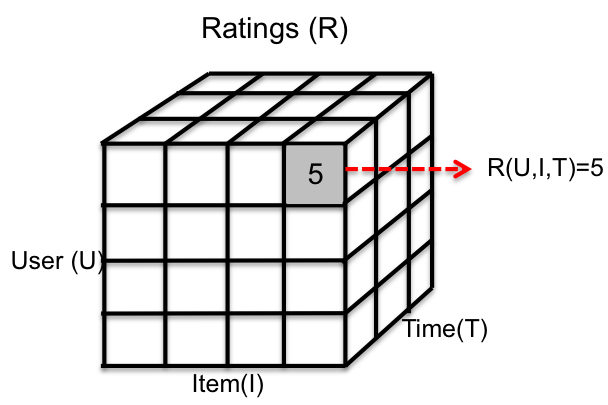
\includegraphics[width=0.40\textwidth]{img/multidimension.png}
\small
\caption{Multidimensional model of context.}
\label{fig:multidimension}   
\end{figure*}

\subsection{Paradigms for using of contextual information}

When recommender system uses contextual information, it starts
with the data having the form \textit{U * I * C * R}, where \textit{C}
is additional contextual dimension and end up with a list of
contextual recommendations $i_{1}$,$i_{2}$,$i_{3}$...$i_{n}$ for each
user. However, when the recommendation process does not take into
account  contextual information, is posible to apply the
information about the current (or desired) context \textit{c} in
various stages of the recommendation process.
Adomavicious\cite{adomavicius2011context} defines three paradigms for
the context-aware recommendation process that is based on contextual
user preference:
\begin{itemize}
\item \textbf{Contextual pre-filtering (or contextualization of
recommendation input).} The approach uses contextual information to
select the most relevant 2D (Users x Items) data for generating
recommendations. One major advantage of this approach is that it
allows deployment of any of the numerous traditional recommendation
techniques previously proposed in the literature\cite{adomavicius2005toward}.
In particular, when using this approach, context
\textit{c} essentially serves as a query (or a filter) for selecting
relevant rating data. An example of a contextual data filter for a
movie recommender system would be: if a person wants to see a movie on
Saturday, only the Saturday rating data is used to recommend movies.
Note that this example represents a crisp pre-filter because the data
was filtered using exactly the specified context (figure
\ref{fig:paradigms}.a).
\item \textbf{Contextual post-filtering (or contextualization of
recommendation output).} In this approach context information
in the input data is ignored when generating recommendations, that is, when
generating the ranked list of all candidate items from which any
number of \textit{top-N} recommendations can be made. Instead,  the
contextual post-filtering approach uses contextual information to
adjust the obtained recommendation list for each user. The
recommendation list adjustments can be made by: (1) filtering out
recommendations that are irrelevant in a given context, or (2)
adjusting the ranking of recommendations in the list. For example, in
a movie recommendation application, if a person wants to see a movie
on a weekend, and if on weekends he or she only watches comedies, the
system can filter out all noncomedies from the recommended list
(figure \ref{fig:paradigms}.b).
\item \textbf{Contextual modeling (or contextualization of
recommendation function).} This approach uses contextual information
directly in the recommendation function as an explicit predictor of a
user's rating for an item and, thus, gives rise to truly
multidimensional recommendation functions representing either
predictive models (such as decision trees, regression, and so on) or
heuristic approaches that incorporate contextual information in
addition to the user and item data (figure \ref{fig:paradigms}.c).\\
\end{itemize}
\begin{figure*}
\captionsetup{font=footnotesize}
\centering
\fbox{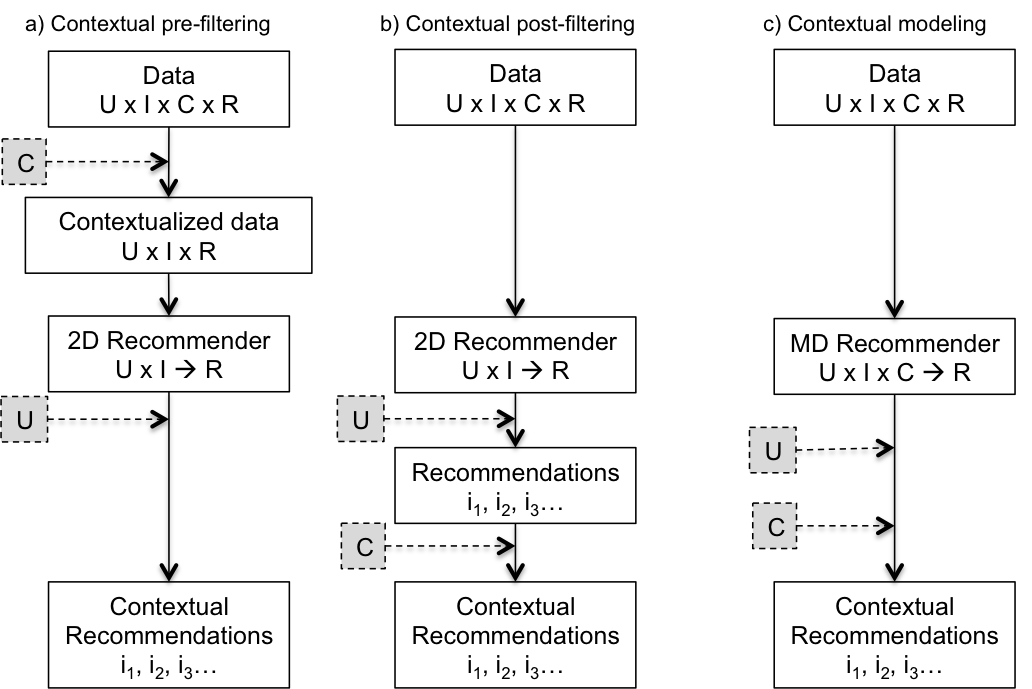
\includegraphics[width=0.80\textwidth]{img/paradigms.png}}
\small
\caption{Paradigms for incorporating context in recommender 
systems\cite{adomavicius2011context}.}
\label{fig:paradigms}   
\end{figure*}







